\documentclass[a4paper]{article}
\usepackage{booktabs} % 引入booktabs包以使用\toprule, \midrule 和 \bottomrule
\usepackage{student}
\usepackage{ctex}
\usepackage{amsmath} 
\usepackage{amsthm}
\usepackage{multirow}
\usepackage{multicol}
\usepackage{listings}
\usepackage[linesnumbered, noend, ruled]{algorithm2e}
% \usepackage{subcaption}
\usepackage{caption}
\usepackage{hyperref}
\usepackage{graphicx}
% \usepackage{float}
\renewcommand*{\proofname}{Proof}
\usepackage{pgf}
% Metadata
\date{\today}
\setmodule{CS64001: Convex Optimization}
\setterm{Spring, 2023}

%-------------------------------%
% Other details
% TODO: Fill these
%-------------------------------%
\title{Assignment 2}
\setmembername{刘建}  % Fill group member names
\setmemberuid{22B903037}  % Fill group member uids (same order)

%-------------------------------%
% Add / Delete commands and packages
% TODO: Add / Delete here as you need
%-------------------------------%
\usepackage{amsmath,amssymb,bm}

\newcommand{\KL}{\mathrm{KL}}
\newcommand{\R}{\mathbb{R}}
\newcommand{\E}{\mathbb{E}}
\newcommand{\T}{\top}

\newcommand{\expdist}[2]{%
        \normalfont{\textsc{Exp}}(#1, #2)%
    }
\newcommand{\expparam}{\bm \lambda}
\newcommand{\Expparam}{\bm \Lambda}
\newcommand{\natparam}{\bm \eta}
\newcommand{\Natparam}{\bm H}
\newcommand{\sufstat}{\bm u}

% \setlength{\parindent}{20pt}
% Main document
\begin{document}
    % Add header
    \header{\href{https://github.com/hitcslj/HIT-CS-Master/tree/main/convex_optimizer/homework/hm2}{all code can be found here: hitcslj/HIT-CS-Master}}
    
    \subsection*{T0}

    \begin{table}[h!]
    \centering
    \begin{tabular}{ccc}
        \toprule
        function  & Minimum value  & Minimum point \\
        \midrule
        Ackley & 0.0 & [0,0] \\
        Booth & 0.0 & [1.0,3.0] \\
        Branin & 0.4 & [-3.14,12.27] \\
        Flower &  0.0 & [0,0] \\
        Michalewicz &  -1.6 & [2.2,2.2] \\
        Rosenbrock Banana & 0.0 & [1.0,1.0] \\
        Wheeler & -1.0 &  [1.0,1.5]\\
        \bottomrule
    \end{tabular}
    \caption{尝试各个方法在 8 个测试函数上的性能表现(只尝试了七个),只需要在代码中体现即可)}
    \end{table}
    

    \subsection*{T1}
    
    \begin{table}[h!]
    \centering
    \begin{tabular}{cccc}
        \toprule
        method  & Minimum value & Minimum point & iterations \\
        \midrule
        共轭梯度法 & -1.25 & [-1.0,1.5] &  2 \\
        \bottomrule
    \end{tabular}
    \caption{用共轭梯度法求解问题}
    \end{table}


    \subsection*{T2}

    分别使用黄金分割,斐波那契算法,二分法和Dichotomous解下列问题:
    如表4,表5
    
    \begin{table}[h!]
    \centering
    \begin{tabular}{cccc}
        \toprule
        method  &  Minimum point & Minimum value & iterations \\
        \midrule
        Golden Section Search & 0.26 & -1.12 & 8 \\
        Fibonacci Searchh & 0.26 & -1.12 & 7 \\
        Bisection Search & 0.23 & -1.12 & 6 \\
        Dichotomous Search & 0.25 & -1.12 & 7 \\
        Shubert-Piyavskii (L = 5) & -0.03 & -0.97 & 3 \\
        \bottomrule
    \end{tabular}
    \caption{Problem a:使用黄金分割求解问题}
    \end{table}


    \begin{table}[h!]
    \centering
    \begin{tabular}{cccc}
        \toprule
        method  &  Minimum point & Minimum value & iterations \\
        \midrule
        Golden Section Search & 3.61 & -39.88 & 12 \\
        Fibonacci Searchh & 3.61 & -39.88 & 12 \\
        Bisection Search & 3.59 & -39.88 & 9 \\
        Dichotomous Search & 3.59 & -39.88 & 10\\
        Shubert-Piyavskii (L = 150) &  0 & -1.0 & 1 \\
        \bottomrule
    \end{tabular}
    \caption{Problem b:使用斐波那契算法求解}
    \end{table}
 

    \subsection*{T3}
    使用不精确的一维搜索算法Goldstein,Goldstein-Price,Wolfe-Powell方法解下列问题 $\min f(x+\lambda d)$:
    \begin{align*}
        f(x) = 100(x_2-x_1^2)^2+(1-x_1)^2, x_1 = (-1,1)^T, d=(1,1)^T 
    \end{align*}

    \begin{table}[h!]
    \centering
    \begin{tabular}{ccc}
        \toprule
        method  &  lambda & iterations\\
        \midrule
        Goldstein & 1.0 & 20\\
        Goldstein-Price & 0.0 & 8\\
        Wolfe-Powell & 0.0 & 8 \\
        \bottomrule
    \end{tabular}
    \caption{使用不精确的一维搜索算法Goldstein,Goldstein-Price,Wolfe-Powell方法}
    \end{table}


    \subsection*{T4}
    计算凸函数的次微分
    (1) $f(x_1, x_2, x_3) = max(|x_1|, |x_2|, |x_3|)$, 在点$(0,0,0)$处. 
        由次梯度定义$\partial f = {g | g^t(y-x) \le f(y)-f(x)} \forall y \in \mathbf{dom} f$,

        \begin{align*}
            f(\mathbf{x}) &\ge f(\mathbf{0})+ \mathbf{g^t} \mathbf{x} \\
            \max \{ |\mathbf{x}| \} &\ge 0 + \mathbf{g^t} \mathbf{x}  \\
            \max \{ |\mathbf{x}| \} &\ge  \mathbf{g^t} \mathbf{x} 
        \end{align*}
        
        故有:$|| g||_1 \le \mathbf{1}$

        注:无穷范数的对偶范数是1-范数.

    (2) $f(x) = e^{|x|}$, 在$x=0$处\dots
        
        \begin{equation*}
            f(x) \ge f(0) + gx \leftarrow
            \begin{cases}
                x>0 \quad \quad g < \frac{e^x -1 }{x} \quad s.t. g< \lim_{x \to 0^+}\frac{e^x -1 }{x}  = 1\\
                x<0 \quad \quad g > \frac{e^{-x} -1 }{x} \quad s.t. g> \lim_{x \to 0^-}\frac{e^{-x} -1 }{x} = -1 \\
            \end{cases} 
        \end{equation*}

        所以次梯度g = $[-1,1]$
        
    (3) $f(x_1, x_2) = max (x_1+x_2-1, x_1-x_2+1)$, 在点$(1,1)$处,
        由subgradient basic calculus rules and pointwise maximum property可得:
        \begin{gather*}
            \partial f = conv \cup_{i \in I(x)} \partial f_i(x) \\
            \partial f_1(x) = A_1 , \quad A_1 = (1, 1)^T \\
            \partial f_2(x) = A_2 , \quad A_2 = (1, -1)^T \\
        \end{gather*}

    \subsection*{T5}
        DFP方法求解问题:$\min 10*x_1^2 + x_2^2 $, $H^{(0) = I}, x^{(0)} = (0.1,0)^T$. 精确一维搜索. 
        \begin{table}[h!]
        \centering
        \begin{tabular}{cccc}
            \toprule
            method  &  Minimum point & Minimum value & iterations  \\
            \midrule
            DFP & [-0.0  0.0] & 0.0 & 2\\
            \bottomrule
        \end{tabular}
        \caption{DFP方法求解问题}
        \end{table}

    \subsection*{T6}
        使用BFGS求解问题 : $\min x_1^2 + 4x_2^2-4x_1 -8x_2$, $H^{(0) = I}, x^{(0)} = (0,0)^T$. 精确一维搜索. 

        \begin{table}[h!]
        \centering
        \begin{tabular}{cccc}
            \toprule
            method  &  Minimum point & Minimum value & iterations  \\
            \midrule
            BFGS & [2.0 1.0] & -8.0 & 2\\
            \bottomrule
        \end{tabular}
        \caption{BFGS方法求解问题}
        \end{table}

    \subsection*{T7}
        分别使用DFP,BFGS,FR conjugate 解优化问题, 并比较算法的优缺点. 
        
        分析:

        DFP法和BFGS法都是拟牛顿法,主要是为了解决牛顿法中Hesse逆矩阵不可解的问题。可以验证的,DFP法和BFGS法提出的矫正矩阵能够得到
        满足拟牛顿条件的矩阵。
        
        拟牛顿条件:
        \begin{align*}
            p^k &= x^{k+1}- x^{k} \\
            q^k &= g^{k+1}- g^{k} \\
            p^k &= H_{k+1}q^k \\ 
        \end{align*}

        DFP提出的矫正矩阵为:

        \begin{equation*}
            H_{k+1} = H_{k} + \frac{p^(k)p^{(k)T}}{p^(k)q^{(k)T}} - \frac{H_kq^{(k)}q^{(k)T H_k}}{q^{(k)T} H_k q^{(k)}}
        \end{equation*}

        可以验证的DFP法构造的$H_k$矩阵都是对称正定矩阵,故每次搜索方向均是函数下降方向。
        在目标函数是二次函数$f(x) = \frac{1}{2}x^TAx+b^Tx+c$时,
        可以证明DFP法构造的搜索方向是关于$A$的一组共轭方向,有限步迭代收敛至极值点。

        和DFP法直接估计Hesse的逆矩阵不同,BFGS法的想法是先估计Hesse矩阵本身,然后经过变换,可以得到BFGS法的矫正公式:
        \begin{equation*}
            H_{k+1}^{BFGS} = H_{k} + (1+ \frac{q^{(k)T}H_kq^{(k)}}{p^{(k)T}q^{(k)}})\frac{p^{(k)}p^{(k)T}}{p^{(k)T}q^{(k)}}
            - \frac{p^{(k)}q^{(k)T}H_k + H_kq^{(k)}p^{(k)T}}{p^{(k)T}q^{(k)}}
        \end{equation*} 

        实际计算经验表明BFGS法的数值稳定性更好。拟牛顿算法是\textbf{无约束优化问题}中最有效的一类算法,在实际计算中规避了二次导数的计算(用一阶导数近似),
        当构造的$H_k$正定时,搜索方向都是下降方向,且具有二次终结性,对于更一般的情况,具有超线性的收敛速度。但是,拟牛顿法需要较大的存储空间,在求解大型
        问题可能会遇到困难。

        FR-conjugate法是一类共轭梯度法,实际是改造了最速下降法,对于目标函数是二次函数的情况,
        在计算$x^{(k+1)}$出梯度方向后,并不直接将搜索方向$d_{k+1}$定为负梯度$-g_{k+1}$方向,而是利用了上次搜索方向$d_{k}$,使得$d_{k+1}, d_{k}$
        是关于$A$的一组共轭方向。这样做的好处在于,可以利用共轭方向的性质,算法具有二次终结性,有限次迭代可收敛。

        和拟牛顿法相比,共轭方向法的优点在于存储量较小, 在求解大型优化问题时占优势。 

        \begin{table}[h!]
            \centering
            \begin{tabular}{cccc}
                \toprule
                method  &  Minimum point & Minimum value & iterations  \\
                \midrule
                DFP & [-1.   1.5] & -1.25 & 2 \\
                BFGS & [-1.   1.5] & -1.25 & 2\\
                FR & [-1.   1.5] & -1.25 & 2 \\
                \bottomrule
            \end{tabular}
            \caption{DFP,BFGS,FR conjugate方法求解问题}
            \end{table}
    \subsection*{T8}
    \textbf{无约束优化问题求解基本思想:}

    无约束优化问题的求解主要有两大类算法:
    \begin{itemize}
        \item  一类是利用导数信息的算法,包括最速下降法,牛顿法,共轭梯度法,拟牛顿法。
    这类方法是利用梯度信息,来选取合适的搜索方向,搜索方向要要满足使得函数值下降的要求。
        \item  另一类算法是不利用导数信息的直接优化方法,包括模式搜索,Rosenbrock法,单纯形搜索,Powell方法等,实际上是根据规则
    在空间中挑选线性无关的搜索方向,自然地,这类方法对于求解变量不多的优化问题比较有效。
    \end{itemize}
    
    一般而言,无约束优化问题的求解涉及两个关键的问题,一个是确定当前点的搜索方向,二是确定搜索步长。


    \textbf{如何将非凸优化问题转化成凸优化问题:}

    首先需要说明相比于非凸问题,凸问题的优势。
    对于凸问题,局部最优解就是全局最优解(更准确的说法是严格凸函数),同时,非凸问题的困难在于在高维空间中,存在许多鞍点(梯度为零,但是
    Hesse矩阵不定)。

    回顾凸问题的定义,需要满足两个条件(1)问题的可行域是一个凸集(2)目标函数是可行域上的一个凸函数。

    在非凸问题转化成凸问题的过程中可以从这两个方向入手:
    \begin{itemize}
        \item 修改目标函数,使其成为一个凸函数,这样就可以满足条件(1)。
        \item 抛弃一些约束条件,或者对约束条件做松弛处理,使得新的可行域是凸集,同时包含原可行域的所有点。
    \end{itemize}




    

\textbf{如何将有约束问题转化成无约束优化问题:}

    可以将对于可行域的约束条件作为惩罚项加入到原目标函数中,比如常见的罚函数方法(内点法,外点法);同时为了解决
    罚函数方法中的缺陷,提出了增广拉格朗日方法。

    \subsection*{T9}
    \textbf{总结最速下降法,牛顿法,修正牛顿法的统一公式描述:}

    \begin{equation*}
        x^{k+1} = x^{k} - \lambda_k d^{k}
    \end{equation*}

    其中,$\lambda_k$ 是每次迭代的步长,$d^{(k)}$ 是每次迭代的搜索方向。
    对于上述方法:

    \begin{itemize}
        \item 最速下降法: 搜索方向是$-\nabla f(x^k)$,可以通过方向导数来证明负梯度是在$x^k$点局部下降最快的方向
        (并非全局下降最快的方向), 每次迭代步长可以通过一维搜索方法确定最优的$\lambda_k$。
        \item 牛顿法: 搜索方向是$-\nabla^2 f(x^k)^{-1} \nabla f(x^k)$, 每次迭代步长为1。牛顿法的基本思想是$x^k$点附近用
        二阶的泰勒展开,用二次函数的极值点近似目标函数的极值点,但是如果$x^k$不满足前提,搜索方向不能保证是下降方向。
        \item 修正牛顿法:牛顿法存在的问题是Hesse的逆矩阵不一定可解,且迭代步长为定值。修正牛顿法的思想是(1)修正Hesse矩阵为
        $B_k = \nabla^2f(x^k) + \epsilon I$,同时用一维搜索方法确定最优的$\lambda_k$。
    \end{itemize}

    \textbf{变尺度法的基本思想:}

    和修正牛顿法不同,变尺度法通过秩2近似,直接求解Hesse矩阵的逆矩阵的近似矩阵$H_k$, 使得近似矩阵$H_k$满足拟牛顿条件
    然后用一维搜索算法确定搜索步长。
    \begin{align*}
        p^k &= x^{k+1}- x^{k} \\
        q^k &= g^{k+1}- g^{k} \\
        p^k &= H_{k+1}q^k \\ 
    \end{align*}

    \subsection*{T10}
    随机梯度下降改良算法求解上述问题:
    
    选取T5中的优化问题,选择用带有动量的梯度下降优化,优化结果如下表所示:
    \begin{table}[h!]
        \centering
        \begin{tabular}{cccc}
            \toprule
            method  &  Minimum point & Minimum value & iterations  \\
            \midrule
            mometum & [0.   0] & 0 & 207\\
            \bottomrule
        \end{tabular}
        \caption{带有动量的梯度下降优化方法求解问题}
        \end{table}



    \subsection*{T11}
    自己查看已有的深度学习模型,训练中其参数的变化是否服从低维特性?尝试画出这些变化的分布:
    % \begin{itemize}
    %     \item Define a new model ResNet18Activations to extract activations from a pre-trained ResNet-18 model.\\
    %     \item Load the CIFAR-10 dataset and create DataLoader objects.\\
    %     \item Extract activations from the ResNet-18 model for the CIFAR-10 dataset.\\
    %     \item Apply PCA and t-SNE on the activations to obtain low-dimensional representations.\\
    %     \item Visualize the low-dimensional representations using matplotlib.
    % \end{itemize}
    效果如下图所示:\\

    \begin{figure}[h!]
        \centering
        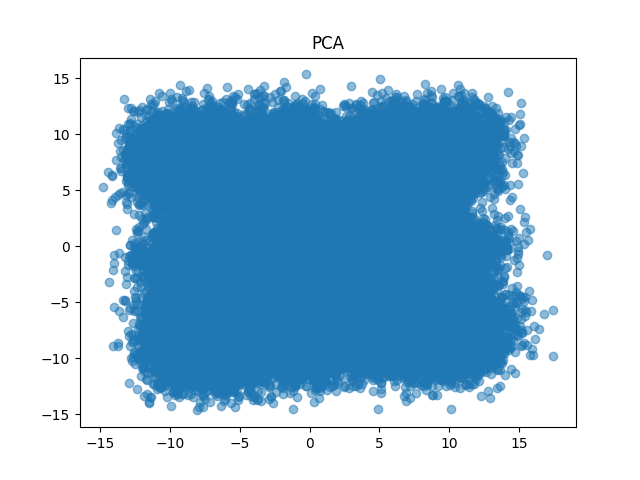
\includegraphics[width=0.5\linewidth]{./figures/pca.png}
        \caption{ResNet-18 activations-PCA}
        \label{fig:pca}
    \end{figure}

    \begin{figure}[h!]
        \centering
        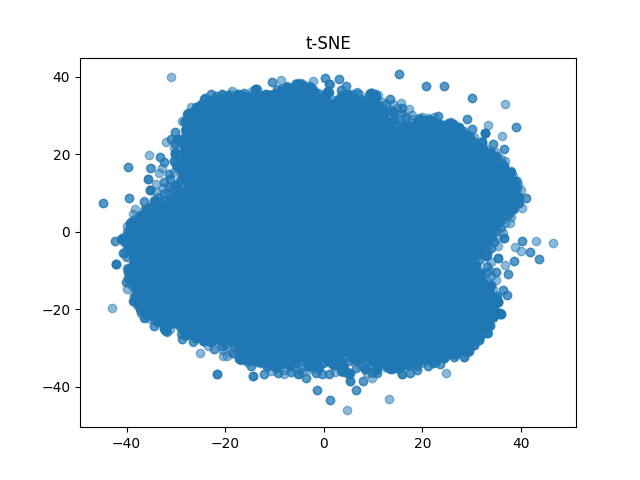
\includegraphics[width=0.5\linewidth]{./figures/tsne.png}
        \caption{ResNet-18 activations-t-SNE}
        \label{fig:tsne}
    \end{figure}


    \subsection*{T12}
    一阶优化算法的加速算法思想(参考林宙晨老师讲义)。

    paper: \url{https://zhouchenlin.github.io/Publications/2020-PIEEE-Review.pdf}

    book: \url{https://link.springer.com/content/pdf/10.1007/978-981-15-2910-8.pdf}


    主要可以从以下个方面考虑:
    \begin{itemize}
        \item 随机梯度:对于较大规模数据,可以通过随机选取一定量的样本数据计算梯度,达到减少计算量的目的。
        \item 动量加速:考虑最速下降法在由于相邻两次的搜索方向正交,导致在最优点附近出现zig-zag现象。考虑用利用上一步的
        梯度信息加速收敛。
        \item Nesterov动量加速:考虑动量加速算法中,梯度变化滞后于函数变化,故需要预测下一时刻的梯度,来修正动量。
    \end{itemize}


    \subsection*{T12}

    思考共轭函数和对偶性的关系。

    参考:\url{https://zhuanlan.zhihu.com/p/265522736}\\
    \url{https://zhuanlan.zhihu.com/p/107483229}

    对偶函数:任意适当函数$f$的对偶函数定义为
    \begin{equation*}
        f^*(y) = \sup_{x \in \mathbf{dom} f} \{ y^Tx - f(x)\}
    \end{equation*}

    根据凸函数的保凸运算, 可以知道共轭函数$f^*(y)$是凸函数。通过共轭函数的定义,容易得到Fenchel不等式即
    \begin{equation*}
        f(x) \ge y^Tx - f^*(y) = g(x,y)
    \end{equation*}

    在上式中,任意的y都能得到一个对$f(x)$下界的刻画。面对$f(x)$非凸的场景,可以通过将目标函数设置为
    $f^{**}$, 即考虑原问题共轭的共轭,此时$f^{**}$是一个凸函数,求解该问题,可以得到原非凸问题最优解
    的一个下界。

    注:’共轭‘之名是指原函数和共轭函数之间的关系是相互的,对于凸问题$f$,其共轭函数的共轭即$f^*$的共轭是$f$。

    共轭函数和拉格朗日对偶函数之间关系密切。考虑一个带约束的优化问题:

    \begin{equation*}
        \min f_0(x) \quad f: R^n \leftarrow R \quad \quad \text{s.t.} 
        \begin{cases}
            Ax \le b, \quad  g: R^m \leftarrow R^n\\
            Cx=0, \quad  h: R^n \leftarrow R^l
        \end{cases}
    \end{equation*}  

    首先可以写出原问题的拉格朗日对偶函数:

    \begin{equation*}
        g(u, v) = \inf_{x \in \mathbf{dom} f} \{ f_0(x) + u^T (Ax-b) + v^TCx\} 
    \end{equation*}

    可以将上式改写成下面的形式:

    \begin{align*}
        g(u,v) &= -b^Tu + \inf_x \{ f_0(x) + (A^Tu+C^Tv)x\} \\
        &= -b^Tu - \sup_x \{ - (A^Tu+C^Tv)x - f_0(x)\} \\
        &= -b^Tu - f^*\{ - (A^Tu+C^Tv)\} 
    \end{align*}


\end{document}
